\subsection{Fundaments of the four color theorem}

The proof of the four color theorem follows the same structure as the five color theorem. We show that every planar graph contains a subgraph that allows us to reduce the coloring problem to a smaller graph. This notion of a \textit{subgraph} of a graph requires some extra attention, since there are multiple ways to be a subgraph.

Given a subgraph $\confg$ of a planar graph $G$. There are roughly two ways that $\confg$ can be a subgraph of $G$. See Figure \ref{fig:containtut}.

\begin{figure}[!ht]
    \centering
    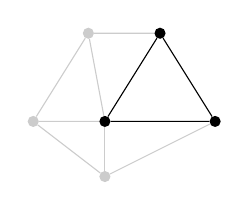
\begin{tikzpicture}[scale=0.7]
        \node[circle, fill, scale=0.015cm] (l1) at (-1, 0) { };
        \node[circle, fill, scale=0.015cm] (l2) at (1, 0) { };
        \node[circle, fill, scale=0.015cm] (l3) at (0, 1.6) {};

        \node[circle, fill, scale=0.015cm, opacity=0.2] (e1) at (-1.3, 1.6) { };
        \node[circle, fill, scale=0.015cm, opacity=0.2] (e2) at (-2.3, 0) { };
        \node[circle, fill, scale=0.015cm, opacity=0.2] (e3) at (-1, -1) { };

        \draw (l1) -- (l2) -- (l3) -- (l1);
        \draw[opacity=0.2] (e1) -- (l1) -- (e2);
        \draw[opacity=0.2] (e3) -- (l1);
        \draw[opacity=0.2] (l3) -- (e1) -- (e2) -- (e3) -- (l2);
    \end{tikzpicture}
    \hspace{1cm}
    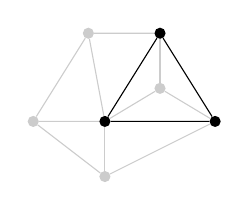
\begin{tikzpicture}[scale=0.7]
        \node[circle, fill, scale=0.015cm] (l1) at (-1, 0) { };
        \node[circle, fill, scale=0.015cm] (l2) at (1, 0) { };
        \node[circle, fill, scale=0.015cm] (l3) at (0, 1.6) {};

        \node[circle, fill, scale=0.015cm, opacity=0.2] (e1) at (-1.3, 1.6) { };
        \node[circle, fill, scale=0.015cm, opacity=0.2] (e2) at (-2.3, 0) { };
        \node[circle, fill, scale=0.015cm, opacity=0.2] (e3) at (-1, -1) { };

        \node[circle, fill, scale=0.015cm, opacity=0.2] (w1) at (0, 0.6) { };

        \draw (l1) -- (l2) -- (l3) -- (l1);
        \draw[opacity=0.2] (w1) -- (l1);
        \draw[opacity=0.2] (w1) -- (l2);
        \draw[opacity=0.2] (w1) -- (l3);
        \draw[opacity=0.2] (e1) -- (l1) -- (e2);
        \draw[opacity=0.2] (e3) -- (l1);
        \draw[opacity=0.2] (l3) -- (e1) -- (e2) -- (e3) -- (l2);
    \end{tikzpicture}
    \caption{Strong containment (left) is an exact copy of a graph $\confg$ in $G$. Weak containment (right) might have additional vertices on the interior of $\confg$.}
    \label{fig:containtut}
\end{figure}

\begin{definition}
    A planar graph $\confg$ is \emph{strongly-contained} in a graph $G$ if no vertices of $G$ are in the interior of $\confg$. Otherwise, $\confg$ is \emph{weakly-contained}.
\end{definition}

Naturally, the form of containment that we will be working with is strong containment. This gives a clear seperation between the interior and exterior of a contained graph $\confg$. With that, we will define what it means for such a graph $\confg$ to be reducible.

\begin{definition}
    A planar graph $\confg$ is \emph{reducible} in a graph $G$ if $\confg$ being strongly-contained in $G$ implies that the 4-coloring of $G$ can be reduced to the 4-coloring of $G'$ with less vertices. $\confg$ is called a \emph{configuration}.
\end{definition}

Now we are ready to phrase the result that lies at the heart of the four and five color theorem.

\begin{theorem}
    \label{funda1}
    Every planar graph $G$ strongly-contains a configuration $\confg$ that is either $k$-reducible, D-reducible or C-reducible in $G$.
\end{theorem}

From this theorem, a 4-coloring of a planar graph $G_0$ can be found as follows. A worked example of this algorithm can be found in Section \ref{sec:algorithm}.

\begin{enumerate}
    \item Find a reducible configuration $C_n$ in $G_n$.
    \item Reduce the graph $G_n$ to the smaller graph $G_{n+1}$.
    \item If $G_{n+1}$ is the empty graph, color all the intermediate graphs starting from $G_n$ all the way until $G_0$, else, repeat Step 1 on $G_{n+1}$.
\end{enumerate}

This process is indeed the same as the repetition argument we gave in the five color theorem. We will now introduce the first concept of reducibility inspired by the five color theorem. 